% !TEX TS-program = pdflatex
% !TEX encoding = UTF-8 Unicode

% This is a simple template for a LaTeX document using the "article" class.
% See "book", "report", "letter" for other types of document.

\documentclass[11pt]{article} % use larger type; default would be 10pt

\usepackage[utf8]{inputenc} % set input encoding (not needed with XeLaTeX)

%%% Examples of Article customizations
% These packages are optional, depending whether you want the features they provide.
% See the LaTeX Companion or other references for full information.

%%% PAGE DIMENSIONS
\usepackage{geometry} % to change the page dimensions
\geometry{a4paper} % or letterpaper (US) or a5paper or....
\geometry{margin=0.5in} % for example, change the margins to 2 inches all round
% \geometry{landscape} % set up the page for landscape
%   read geometry.pdf for detailed page layout information

\usepackage{graphicx} % support the \includegraphics command and options

% \usepackage[parfill]{parskip} % Activate to begin paragraphs with an empty line rather than an indent

%%% PACKAGES
\usepackage{booktabs} % for much better looking tables
\usepackage{array} % for better arrays (eg matrices) in maths
\usepackage{paralist} % very flexible & customisable lists (eg. enumerate/itemize, etc.)
\usepackage{verbatim} % adds environment for commenting out blocks of text & for better verbatim
\usepackage{subfig} % make it possible to include more than one captioned figure/table in a single float
% These packages are all incorporated in the memoir class to one degree or another...

%%% HEADERS & FOOTERS
\usepackage{fancyhdr} % This should be set AFTER setting up the page geometry
\pagestyle{fancy} % options: empty , plain , fancy
\renewcommand{\headrulewidth}{0pt} % customise the layout...
\lhead{}\chead{}\rhead{}
\lfoot{}\cfoot{\thepage}\rfoot{}

%%% SECTION TITLE APPEARANCE
\usepackage{sectsty}
\allsectionsfont{\sffamily\mdseries\upshape} % (See the fntguide.pdf for font help)
% (This matches ConTeXt defaults)

%%% ToC (table of contents) APPEARANCE
\usepackage[nottoc,notlof,notlot]{tocbibind} % Put the bibliography in the ToC
\usepackage[titles,subfigure]{tocloft} % Alter the style of the Table of Contents
\renewcommand{\cftsecfont}{\rmfamily\mdseries\upshape}
\renewcommand{\cftsecpagefont}{\rmfamily\mdseries\upshape} % No bold!

%%% END Article customizations

%%% The "real" document content comes below...

\title{Week 8 Assignment}
\author{Efeosa Eguavoen - 17324649}
%\date{} % Activate to display a given date or no date (if empty),
         % otherwise the current date is printed 

\begin{document}
\maketitle

\section{i}
\subsection{A}
\subsection{B}
\section{ii}
\subsection{A}
\subsection{B}
\subsubsection{i}
Keras says the model has 37,146 parameters.  The dense layer has the most parameters with 20,490 parameters.  This is because the dense layer is a fully connected layer with each output being a function of the weighted sum of all the inputs. Since this layer can have multiple outputs, it means the number of parameters that need to be learned here increases rather quickly.  It has n*m parameters with n being the length of the input vector and m being the number of output channels. The test data performs significantly worse then the training data in terms of accuracy.  Both classifiers don't perform particularly well,  but when compared to a random classifier, they both still perform significantly better.  I used a random classifier as my baseline to test if the model is actually working and learning the the data properly versus randomly selecting numbers.
\\\\ Accuracy of Test Data: 0.49
\\ Accuracy of Training Data: 0.64
\\ Accuracy of Random Classifier: 0.10
\subsubsection{ii}
From the charts the history variable outputs, it seems that as time goes one the model captures the trends in the data more and more.  Initially it under-fits both the training dataset and the testing dataset, but the test data set performs better.  But after 20 epochs, this switches with the training data performing better than the test data. It seems that the model is much better at predicting to the training data than the testing data.  This is probably due to the model possibly over-fitting to the training data and not being general enough to be able to predict on new data accurately.
\subsubsection{iii}
The prediction accuracy seems to increase slightly with more training data.  The 5K dataset has a lower overall prediction accuracy compared to any of the other datasets.  .The training data accuracy only increases by ~10\% with more training data, with the 40K dataset having an accuracy of 0.74 compared to 0.64 with the 5K dataset.  But the test dataset performs significantly better going to 0.7 with the 40K dataset from 0.49 with the 5K dataset,  an improvement of about 20\%.  From the history plots below, we can see that as we increase the amount of training data, our accuracy increases while our loss decreases.  But it seems the returns decrease more and more as we increase the size of the dataset.  \\
In terms of time taken per step: \\ 5K dataset: 7.2ms/step\\10K dataset: 6.5ms/step\\20K dataset: 1s 06ms/step\\40K dataset: 2s 7ms/step. \\
As the size of out dataset grows, the time taken per step increases, taking about 3x as long for a setp for a dataset that's 8x as big.  The tradeoff here seems to be worth it given the jump in performance for little extra computing time. (I used a GTX 1070 GPU to run this hence the times being low).
\begin{figure}[h]
\centering
\subfloat[5k Dataset]{{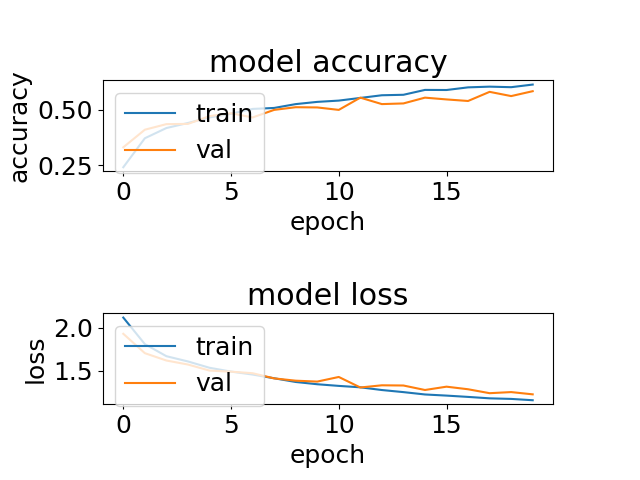
\includegraphics[width=8cm]{5k.png}}}
\qquad
\subfloat[10k Dataset]{{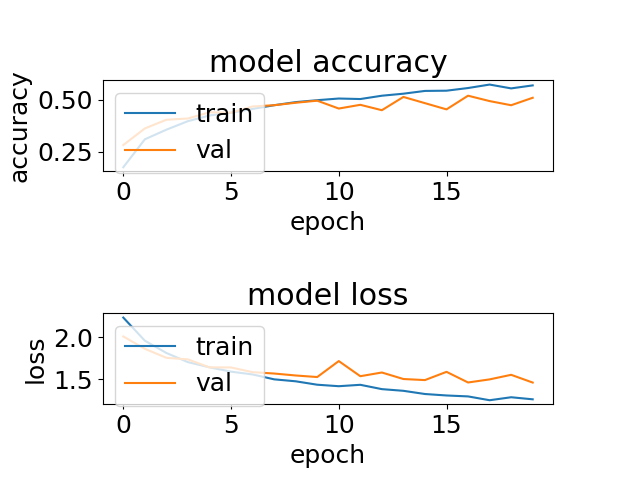
\includegraphics[width=8cm]{10k.png}}}
\qquad
\subfloat[20k Dataset]{{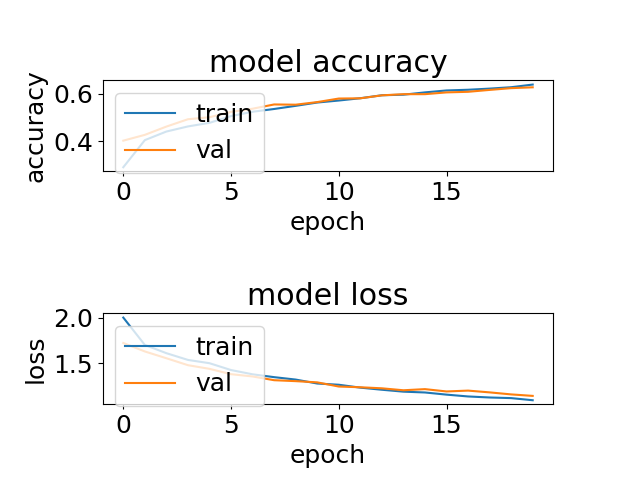
\includegraphics[width=8cm]{20k.png}}}
\qquad
\subfloat[40k Dataset]{{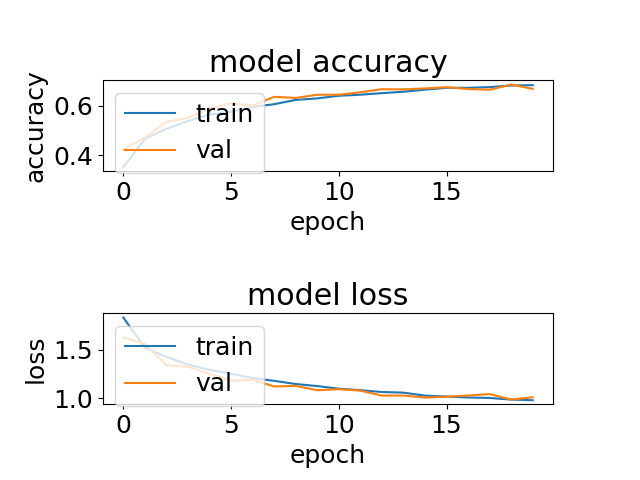
\includegraphics[width=8cm]{40k.png}}}
\qquad
\end{figure}
\subsubsection{iv}
As we vary the L1 penalty,  the accuracy fluctuates quite a bit.  With 0, our accuracy actually increases in terms of the training and test data but as we increase the penalty,  the accuracy become worse and worse.  Using a large L1 value such as 10, out accuracy is terrible got both our training and test datasets. This could be due to the fact that by increasing th L1 penalty, the CNN attempts to prevent overfitting more and more and hence begins underfitting the data with larger values of L1 since the weights are so high.
\begin{figure}[h]
\centering
\subfloat[L1 = 0]{{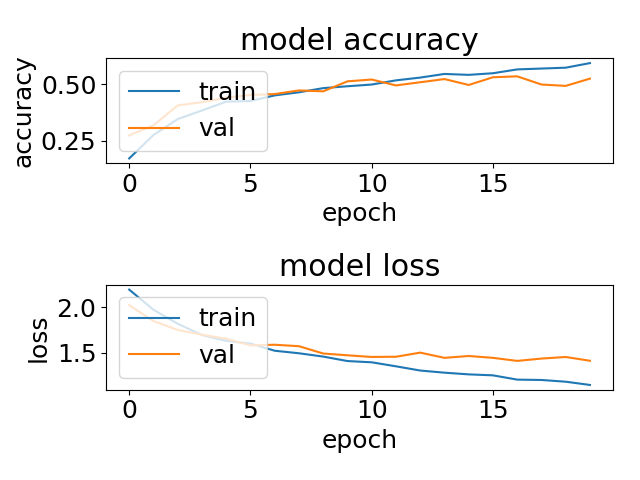
\includegraphics[width=8cm]{L0.png}}}
\qquad
\subfloat[L1 = 0.0001]{{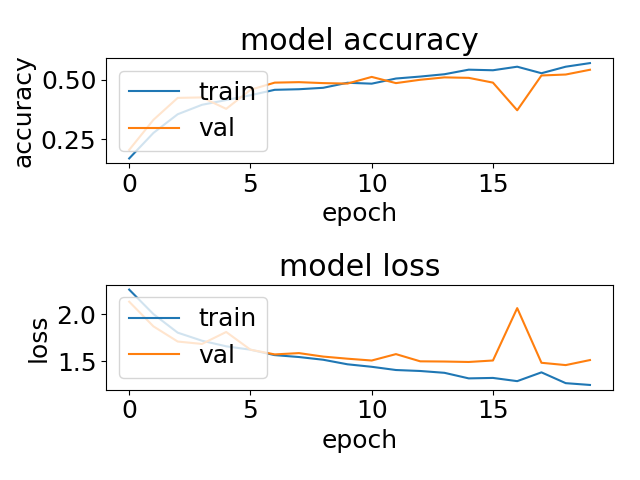
\includegraphics[width=8cm]{L1.png}}}
\qquad
\subfloat[L1 = 0.001]{{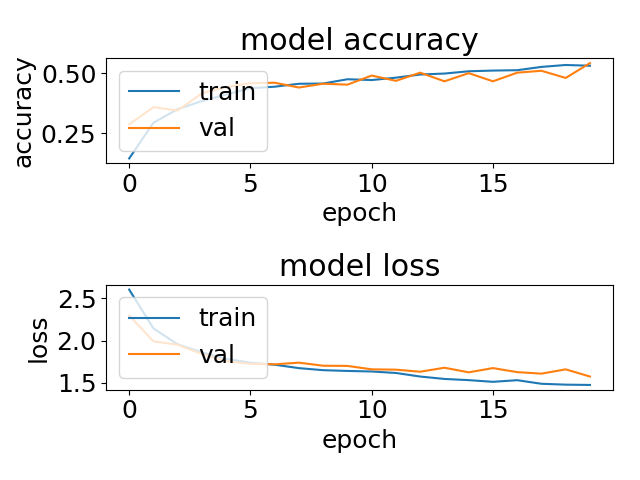
\includegraphics[width=8cm]{L2.png}}}
\qquad
\subfloat[L1= 0.01]{{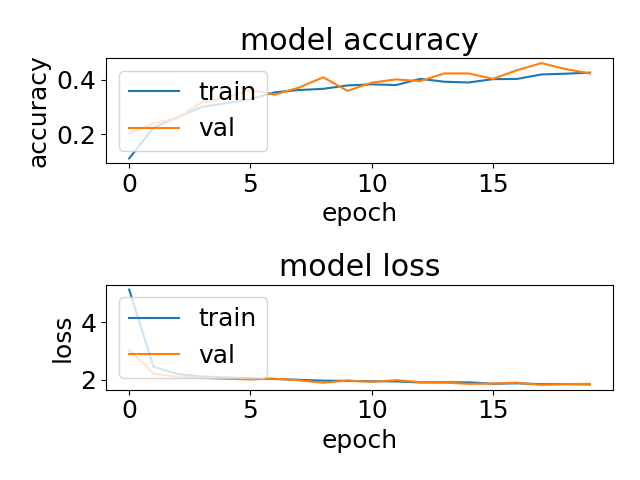
\includegraphics[width=8cm]{L3.png}}}
\qquad
\subfloat[L1 = 0.1]{{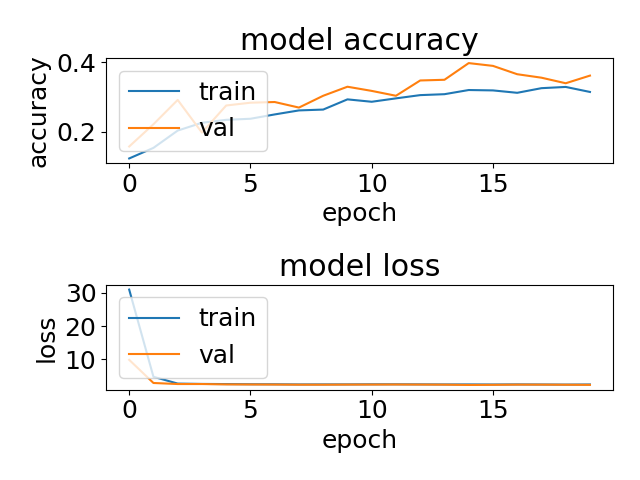
\includegraphics[width=8cm]{L4.png}}}
\qquad
\subfloat[L1 = 1]{{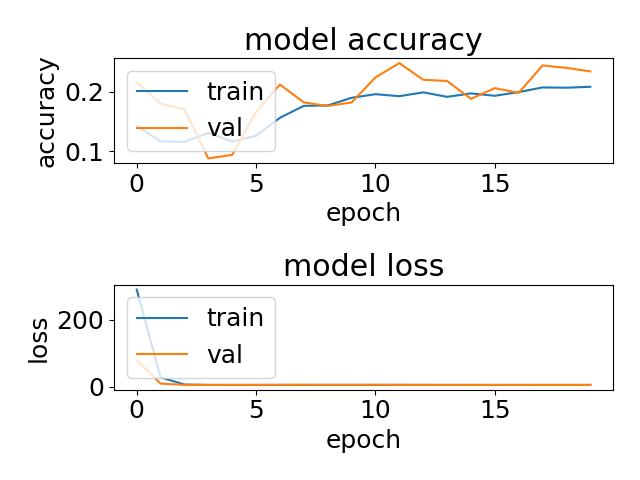
\includegraphics[width=8cm]{L5.png}}}
\qquad
\subfloat[L1 = 10]{{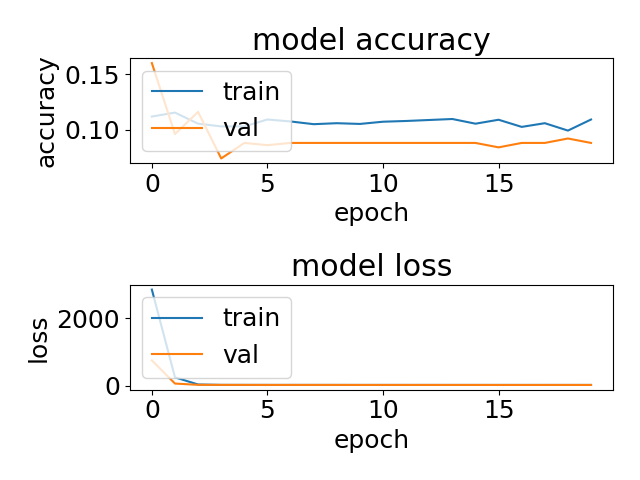
\includegraphics[width=8cm]{L6.png}}}
\end{figure}
\clearpage
\subsection{C}
\end{document}
